\documentclass{article}

\usepackage{listings}
\usepackage{graphicx}

\title{F\'isica at\'omica: Tarea 3}
\author{Iv\'an Mauricio Burbano Aldana}

\begin{document}

\maketitle

Para poder resolver el problema en cuesti\'on se utiliz\'o el siguiente c\'odigo:

\begin{lstlisting}[breaklines = true]

import numpy as np
import matplotlib.pyplot as plt

plt.rc("text", usetex = True)

x = np.linspace(0, 3, 300 + 1)
U0 = 100
res = 100
E_ligado = np.linspace (0, 100, res)
inicial = 1
criterio = 0.014
Epar = []
Eimpar = []

def U(x):
	if(x <= 1):
		return 0
	else:
		return U0

def psi(x, U0, E, paridad, inicial):
	if (paridad == 0):
		phi = [inicial]
		Dphi = [0]
	else:
		phi = [0]
		Dphi = [inicial]
	for n in range(1,len(x)):
			Dphi.append(Dphi[n - 1] + ((U(x[n - 1]) - E) * phi[n - 1] * (x[n] - x[n - 1])))
			phi.append(phi[n - 1] + (Dphi[n - 1] * (x[n] - x[n - 1])))
	return [phi, Dphi]

def buscador(E_iniciales, paridad):
	E = []
	for n in range(0, len(E_iniciales) - 1):
		Dsol1 =  psi(x, U0, E_iniciales[n], paridad, inicial)[1]
		Dsol2 =  psi(x, U0, E_iniciales[n + 1], paridad, inicial)[1]
		if(np.sign(Dsol1[300]) != np.sign(Dsol2[300])):
			E.append(E_iniciales[n])	
			E.append(E_iniciales[n + 1])	
	return E

Epar = buscador(E_ligado, 0)
Eimpar = buscador(E_ligado, 1)

for n in range(0, len(Epar[::2])):
	valor = criterio + 1
	while (abs(valor) > criterio):
		Energias = np.linspace(Epar[2*n], Epar[2*n + 1], res)
		[Epar[2*n], Epar[2*n + 1]] = buscador(Energias, 0)

for n in range(0, len(Eimpar[::2])):
	valor = criterio + 1
	while (abs(valor) > criterio):
		Energias = np.linspace(Eimpar[2*n], Eimpar[2*n + 1], res)
		[Eimpar[2*n], Eimpar[2*n + 1]] = buscador(Energias, 1)
		valor = psi(x, U0, (Eimpar[2*n] + Eimpar[2*n + 1])/2, 1, inicial)[0][300]
		print valor

plt.figure()
plt.title(r"Comportamiento en estados ligados de part\'iculas pares")
for n in range(0, len(Epar) - 1):
	if ((2*n + 1) < len(Epar)):
		E = (Epar[2*n + 1] + Epar[2*n])/2
		phi = psi(x, U0, E, 0, inicial)[0]
		plt.plot(x, phi, label = r"$%f \leq E \leq %f$" % (Epar[2*n], Epar[2*n + 1]))
	else:
		break
plt.ylabel(r"$\psi$", fontsize = 15)
plt.xlabel(r"$x$", fontsize = 15)
plt.legend()
plt.savefig("comportamiento_ligado_par.pdf", format = "pdf") 

plt.figure()
plt.title(r"Comportamiento en estados ligados de part\'iculas impares")
for n in range(0, len(Eimpar) - 1):
	if ((2*n + 1) < len(Eimpar)):
		E = (Eimpar[2*n + 1] + Eimpar[2*n])/2
		phi = psi(x, U0, E, 1, inicial)[0]
		plt.plot(x, phi, label = r"$%f \leq E \leq %f$" % (Eimpar[2*n], Eimpar[2*n + 1]))
	else:
		break
plt.ylabel(r"$\psi$", fontsize = 15)
plt.xlabel(r"$x$", fontsize = 15)
plt.legend()
plt.savefig("comportamiento_ligado_impar.pdf", format = "pdf") 

f, axarr = plt.subplots(2, 2)
axarr[0, 0].set_title(r"$E = 100$")
axarr[0, 0].plot(x, psi(x, U0, 100, 0, inicial)[0], label = "par")
axarr[0, 0].plot(x, psi(x, U0, 100, 1, inicial)[0], label = "impar")
axarr[0, 0].legend()
axarr[0, 0].set_xlabel(r"Posici\'on")
axarr[0, 0].set_ylabel(r"Funci\'on de onda")
axarr[0, 1].set_title(r"$E = 200$")
axarr[0, 1].plot(x, psi(x, U0, 200, 0, inicial)[0], label = "par")
axarr[0, 1].plot(x, psi(x, U0, 200, 1, inicial)[0], label = "impar")
axarr[0, 1].set_xlabel(r"Posici\'on")
axarr[0, 1].set_ylabel(r"Funci\'on de onda")
axarr[1, 0].set_title(r"$E = 700$")
axarr[1, 0].plot(x, psi(x, U0, 700, 0, inicial)[0], label = "par")
axarr[1, 0].plot(x, psi(x, U0, 700, 1, inicial)[0], label = "impar")
axarr[1, 0].set_xlabel(r"Posici\'on")
axarr[1, 0].set_ylabel(r"Funci\'on de onda")
axarr[1, 1].set_title(r"$E = 1000$")
axarr[1, 1].plot(x, psi(x, U0, 1000, 0, inicial)[0], label = "par")
axarr[1, 1].plot(x, psi(x, U0, 1000, 1, inicial)[0], label = "impar")
axarr[1, 1].set_xlabel(r"Posici\'on")
axarr[1, 1].set_ylabel(r"Funci\'on de onda")
f.tight_layout()
plt.savefig("comportamiento_libre.pdf")

\end{lstlisting}

La tecnica consisti\'o en hace un recorrido de "res" valores de energ\'ia entre 0 y 100 (el rango de energias en el que sabemos que se encuentra una part\'icula ligada) para hacer una primera identificaci\'on de valores tentativos. Al principio fue bastante dif\'icil encontrar alg\'un valor. Sin embargo, una vez se encontr\'o que alrededor de 2 hab\'ia uno, se not\'o que cuando se pasa por \'el, el signo de la derivada en el valor $x=3$ cambiaba. En efecto, de un lado del valor que entregaba una funci\'on de onda aceptable la funci\'on crec\'ia en 3 mientras que en el otro la funci\'on decrec\'ia. Por lo tanto se cre\'o la funci\'on "buscador" que toma una lista de valores de energ\'ia y los compara en cadena identificando cuando cambia la derivada de signo. Las dos energ\'ias entre las cuales hay tal cambio se guardan en una lista de manera que sabemos que entre ambas energ\'ias se encuentra una de las permitidas por la teor\'ia cu\'antica.

Una vez se identifican valores tentativos (o mejor dicho, intervalos tentativos) para la energ\'ia (se encontraron 4 para soluciones pares y 3 para soluciones impares) se repite el algoritmo solo que ahora se hace un recorrido sobre cada uno de estos intervalos subdividiendolos una vez m\'as con "res". De esta manera se cierra el intervalo en el cual pueden estar la energ\'ia buscada. Esto se hace de manera iterativa hasta que el valor absoluto de la funci\'on de onda en $x = 3$ es menor a un "criterio" que se determina al comienzo del c\'odigo. Una vez se cumple esto, se grafican las soluciones con la energ\'ias promedio de cada intervalo.

\begin{figure}
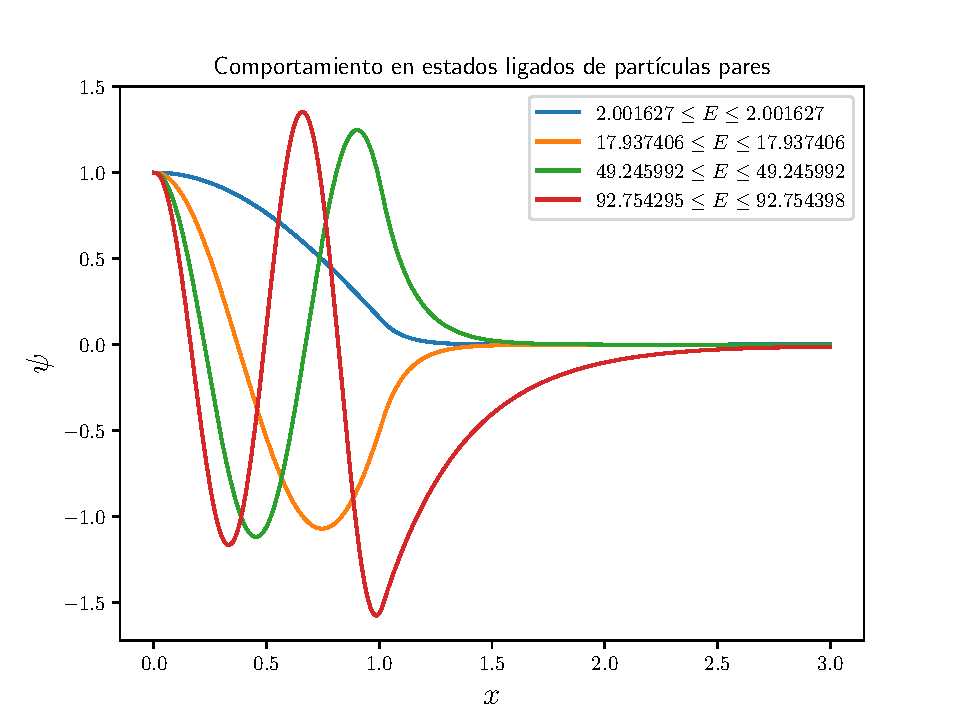
\includegraphics[width = \textwidth]{comportamiento_ligado_par.pdf}
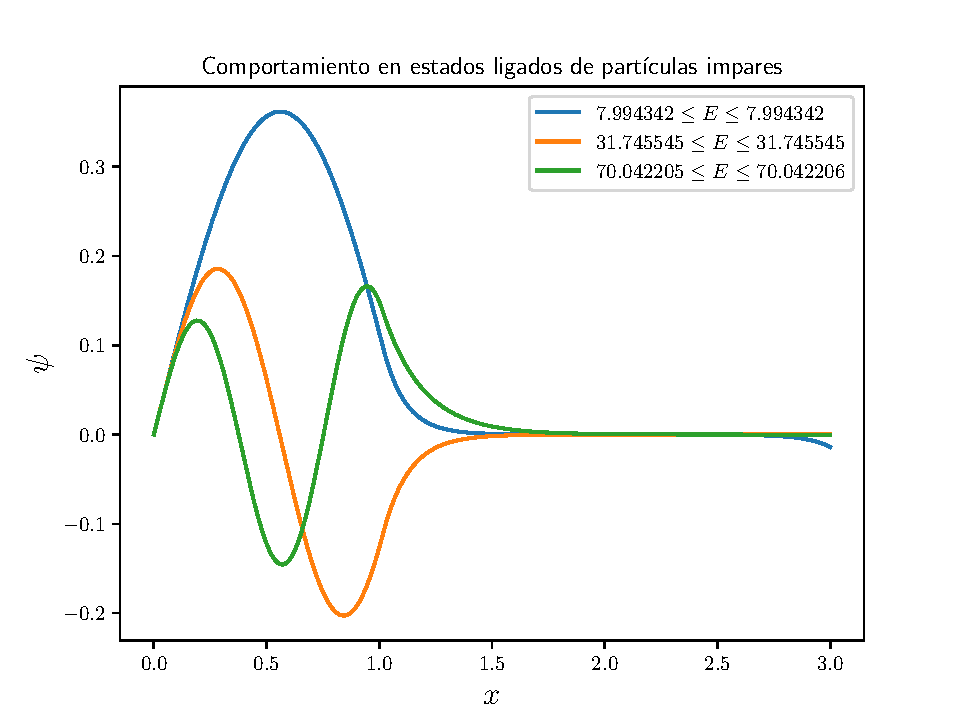
\includegraphics[width = \textwidth]{comportamiento_ligado_impar.pdf}
\caption{Las funciones de onda junto con sus energ\'ias halladas mediante el c\'odigo dise\~nado}
\end{figure} 

Los resultados fueron bastante satisfactorios. El c\'odigo permite hallar los valores de energ\'ia con una presici\'on de hasta 7 cifras significativas en segundos. Ademas, se puede apreciar el comportamiento oscilatorio (de frecuencia constante para aquellas con m\'as de un pico) para $x\leq 1$ seguido de un decaimiento exponencial. Sin embargo, el metodo de integraci\'on usado (regla de Euler) puede mejorarse pues las ondas obtenidas con varios picos no tienen amplitud constante. En resumen, lo que hace a este c\'odigo tan fuerte es el algoritmo "buscador" y su implementaci\'on tanto en la busqueda de valores tentativos de energ\'ia como en el depuramiento de estos.

Por completitud se experiment\'o tambien con valores de energ\'ia mayores a 100.

\begin{figure}
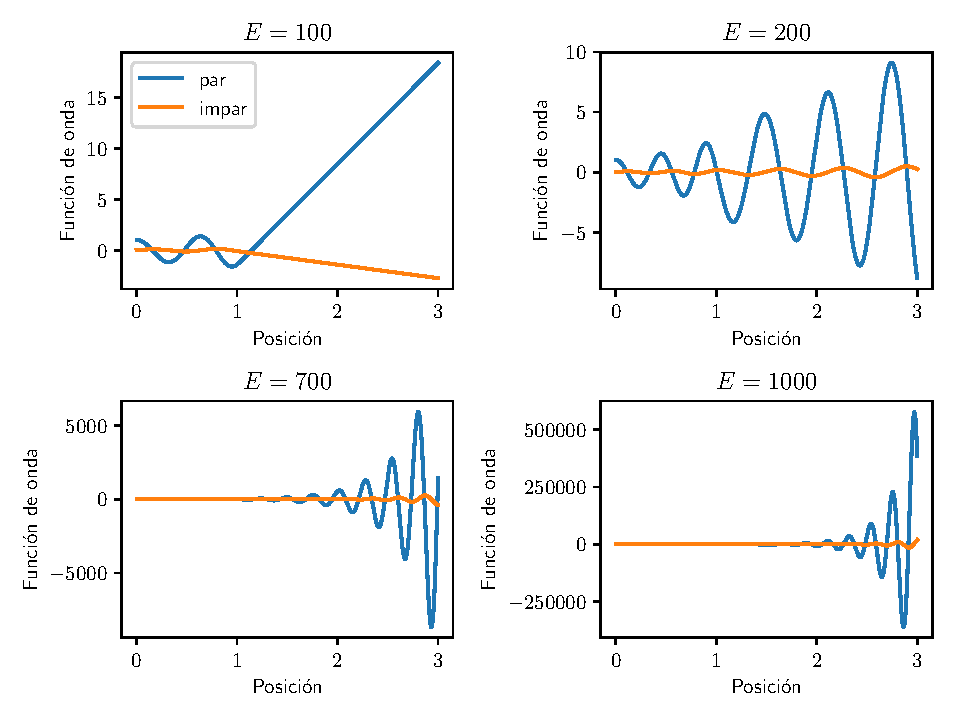
\includegraphics[width = \textwidth]{comportamiento_libre.pdf}
\caption{Funciones de onda libres}
\end{figure}

Se puede observar un comportamiento sinusoidal como es esperado. En particular, para las de menor energ\'ia, se puede observar el cambio en la frecuencia de la onda al salir del pozo de potencial. Notese que estas funciones no son cuadrado integrables y por lo tanto las energ\'ias que les corresponden no son valores propios del hamiltoniano. Este es un ejemplo donde se evidencia que el espectro de un operador (en este caso el hamiltoniano) no necesariamente coincide con sus valores propios.

\end{document}
